\documentclass[12pt]{article}
\usepackage{geometry}                % See geometry.pdf to learn the layout options. There are lots.
\geometry{letterpaper}                   % ... or a4paper or a5paper or ... 
%\geometry{landscape}                % Activate for for rotated page geometry
\usepackage[parfill]{parskip}    % Activate to begin paragraphs with an empty line rather than an indent
\usepackage{daves,fancyhdr,natbib,graphicx,dcolumn,amsmath,lastpage,url}
\usepackage{amsmath,amssymb,epstopdf,longtable}
\usepackage{paralist} 
\DeclareGraphicsRule{.tif}{png}{.png}{`convert #1 `dirname #1`/`basename #1 .tif`.png}
\pagestyle{fancy}
\lhead{CE 3372 -- Water Systems Design}
\rhead{FALL 2020}
\lfoot{EXERCISE 6}
\cfoot{}
\rfoot{Page \thepage\ of \pageref{LastPage}}
\renewcommand\headrulewidth{0pt}



\begin{document}
\begin{center}
{\textbf{{ CE 3372 -- Water Systems Design} \\ {Exercise Set 6}}}
\end{center}

\begingroup
\begin{tabular}{p{1.5in} p{5in}}
Purpose: & Application of Manning's equation and flow geometry in open channels; \\
~ & ~ \\
ABET Criteria 3: & (a) \dots apply knowledge of mathematics, science, and engineering  \\
~ & (e)  \dots solve engineering problems  \\
~ & (k) \dots an ability to use the techniques, skills, and modern engineering tools necessary for engineering practice. \\
%~ & ~ \\
%Grading Criteria:  & Completion; Correct Solutions; Calculation Details \\
\end{tabular}
\endgroup
\section*{\small{Exercises}}

\begin{enumerate}

%%%%%%%%%%%%%%%%%%
\item Water flows at 8$m^3/s$ through a rectangular channel 4 m wide and 3 m deep.  If the velocity is 1$m/s$, calculate the flow depth in the channel.  If this channel expands (downstream) to a width of 5 m and the depth decreases by 0.5 m from the upstream depth, what is the mean section velocity in the expanded section?
\begin{enumerate}[a)]
\item Sketch the two cross sections and label the width, depth, and channel wall height.
\item Write the relationships between velocity, depth, and discharge for each section.
\item Compute the depth in the narrow section.
\item Compute the depth in the wider section.
\item Compute the velocity in the wider section.
\end{enumerate}
\item Water flows at a depth of 2.20 m in a trapezoidal, concrete-lined section with a bottom width of 3.6 m and side slopes of 2:1 (H:V).  The longitudinal slope of the channel is 0.0006 and the water temperature is 293$^o$K. Assuming uniform-flow conditions, estimate the mean section velocity (in meters per second) and the discharge (in cubic meters per second)  in the channel. 
\begin{enumerate}[a)]
\item Sketch the cross section and label the width, depth, and side slope.
\item Write the relationships between velocity, depth, and discharge for the section.
\item Compute the velocity in the section.
\item Compute the discharge in the section.
\end{enumerate}
\clearpage
\item A circular sewer is laid on a slope of 0.5\%.  What diameter is required if the concrete pipe is to carry 25 cubic-feet per second?   If the desired design mean section velocity is between 3 and 7 feet per second, is the design acceptable?
\begin{enumerate}[a)]
\item Sketch the cross section and label the diameter and flow depth.
\item Write the appropriate relationships between velocity, depth, and discharge for the section.
\item Size the pipe; assume pipe is flowing full, but not pressurized.
\item Compute the actual fill depth (the pipe will flow less than full) using either the hydraulic element chart or by computation.
\item Compute the velocity in the section (using the actual fill depth).
\item Is the computed velocity within the stated criteria?
\end{enumerate}

\item A grass-lined roadside swale (ditch) is to be built as a trapezoidal channel to carry 20 cubic-feet per second, with a 1 foot freeboard.   If the desired flow depth is 1 foot, and the right of way available to fit the ditch is 12 feet, what is the required side slope and bottom width.   The longitudinal slope is 1\%.
\begin{enumerate}[i]
\item Sketch the cross section and label the width, depth, and side slope.
\item Write the appropriate relationships between velocity, depth, and discharge for the section.
\item Compute the required side-slope in the section.
\item Compute the mean section velocity in the section.
\end{enumerate}

%\item A square shaped 50 acre, single family residential area in Harris County is graded from an elevation of 150-feet at the corner to 139-feet at the outlet as depicted on Figure \ref{fig:watershed.jpg}.
%
%\begin{figure}[h!] %  figure placement: here, top, bottom, or page
%   \centering
%   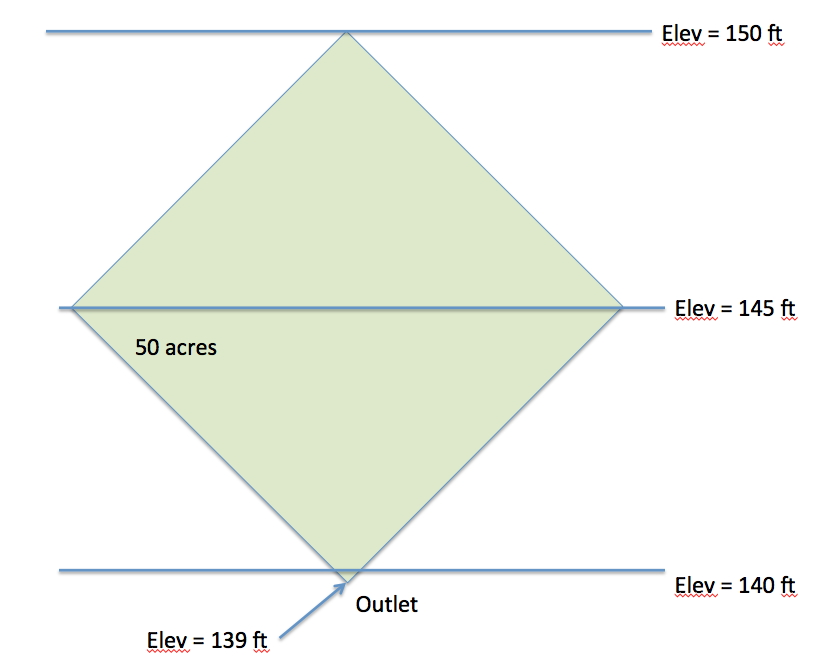
\includegraphics[width=4.8in]{watershed.jpg} 
%   \caption{50 acre square watershed with elevation contour overlay}
%   \label{fig:watershed.jpg}
%\end{figure} 
%\clearpage
%
%\begin{enumerate}[a)]
%\item Draw on the diagram the longest flow path from the highest elevation to the outlet.
%\item Draw on the diagram the shortest flow path from the highest elevation to the outlet.
%\item Determine the length, in feet, of one side (edge) of the sub-catchment.
%\item Determine the length, in feet, of both flow paths.
%\item Determine the average dimensionless slope along each flow path.
%\item Estimate the time of concentration using NRCS upland method.
%\item Using the DDF Atlas, TP-40, or EBDLKUP-2015 estimate the rainfall intensity for a 10-year ARI.
%\item Using (and citing) a runoff coefficient table, specify the runoff coefficient for the sub-catchment.
%\item Estimate the peak discharge for the sub-catchment for a 10-year ARI using the Rational Method.
%\item Determine the diameter of a reinforced concrete pipe to convey the discharge to a receiving stream if the pipe is to be laid on a slope of 0.5\%, and is to flow 1/2 full at the specified discharge.
%\end{enumerate}
%
%\item Using the DDF Atlas, TP-40, or EBDLKUP-2015 estimate the rainfall depth for a 10-year, 6-hour storm in Harris County, Texas.
%
%\item Using the SCS Tabulation or TXHYETO, construct from the 10-year, 6-hour storm a design hyetograph at 15 minute intervals.
%
%\item A drainage area upstream of an inlet will produce a peak discharge of 12 cfs for a design storm appropriate for the location.  
%The longitudinal slope of the roadway is 3.5 ft per 1000 ft, the transverse (cross) slope is 2.0 ft per 100 ft.
%The inlet depression depth is to be 0.35 ft and the depression width is to be 5.0 ft.
%
%Estimate the required curb opening inlet length if carryover flow of 1 cfs is allowed. 
%
%\begin{enumerate}[a)]
%\item Select an appropriate value for Manning's n; cite your source of the value.
%\item Compute the flow depth just upstream of the inlet using HDM Equation 10-1.
%\item Compute ponding width using HDM Equation 10-2.
%\item Compute conveyance in the depressed section using HDM Equation 10-10, 10-11, and 10-9.
%\item Compute conveyance in ``beyond depressed section'' using HDM Equation 10-12, 10-13, and 10-9.
%\item Compute conveyance ratio using HDM Equation 10-8.
%\item Compute equivalent cross slope using HDM Equation 10-14.
%\item Compute inlet capacity as a function of length using HDM Equation 10-15, rearranged to solve for Q in terms of L.
%\item Compare the manual calculations above with the ``Inlet on Grade'' spreadsheet shown on the class server.  Are the results similar, different?  
%\end{enumerate}
%
%\item If the design storm in the previous problem has a rainfall intensity of 3 inches per hour, and the rational runoff coefficient for the area is 0.9, estimate the drainage area contributing to the inlet.

\end{enumerate}
\end{document}  